\documentclass[11pt,a4paper]{article}

\usepackage[margin=2.5cm]{geometry}
\usepackage{amsmath,amssymb,amsthm}
\usepackage{booktabs}
\usepackage{graphicx}

\newtheorem{proposition}{Proposition}[section]
\newtheorem{remark}[proposition]{Remark}

\newcommand{\R}{\mathbb{R}}
\newcommand{\Z}{\mathbb{Z}}
\newcommand{\Q}{\mathbb{Q}}
\newcommand{\N}{\mathbb{N}}

\title{\textbf{Wilson Matching Matrices:\\
at the Top of the Askey Scheme}}
\author{Robin Langer and Claude Code}
\date{August 2026}

\begin{document}
\maketitle

%% ===================================================================
\section{Setup}
%% ===================================================================

The Wilson polynomials sit at the top of the Askey scheme.
On $(0,\infty)$ with parameters $(a,b,c,d)$, the weight is
\[
  W(x) = \biggl|\frac{\Gamma(a{+}ix)\,\Gamma(b{+}ix)\,
  \Gamma(c{+}ix)\,\Gamma(d{+}ix)}{\Gamma(2ix)}\biggr|^2,
\]
and the orthogonal polynomials $p_n(x^2)$, degree~$n$ in~$x^2$, satisfy
(DLMF~18.25)
\[
  \int_0^\infty p_m(x^2)\, p_k(x^2)\, W(x)\, dx = h_n\, \delta_{mk}.
\]
We study the \emph{primary parameters}
$(a,b,c,d) = (\tfrac14, \tfrac14, \tfrac34, \tfrac34)$,
$s = a{+}b{+}c{+}d = 2$, chosen because these pair the
$\Gamma(s/2)$ and $\Gamma((s+1)/2)$ worlds of the Riemann
$\xi$-function.

The weight factors analytically as $W = w_+ \cdot \overline{w_+}$ with
\[
  w_+(x) = \frac{\Gamma(a{+}ix)\,\Gamma(b{+}ix)\,
  \Gamma(c{+}ix)\,\Gamma(d{+}ix)}{\Gamma(2ix)}.
\]
We define matching matrices exactly as in the Meixner--Pollaczek case:
\begin{align}
  b_{mk} &= \frac{1}{h_0}\int_0^\infty p_m\, p_k\; W^{3/2}\, dx,
  \label{eq:bdef} \\
  c_{mk} &= \frac{1}{h_0}\int_0^\infty p_m\, p_k\; w_+\, W\, dx.
  \label{eq:cdef}
\end{align}

%% ===================================================================
\section{A Norm Identity}
%% ===================================================================

The DLMF~18.25 orthogonality uses the weight
$w(y^2) = (1/2y)\,|\prod \Gamma(a_j{+}iy)/\Gamma(2iy)|^2$,
integrating over $y \in (0,\infty)$.  We work instead with the
Pochhammer-free polynomials
\[
  p_n(x^2) = {}_4F_3\!\bigl({-}n,\, n{+}s{-}1,\, a{+}ix,\, a{-}ix;\;
  a{+}b,\, a{+}c,\, a{+}d;\; 1\bigr)
\]
and the ``bare'' inner product
$\langle f, g \rangle = \int_0^\infty f(x)\, g(x)\, W(x)\, dx$
(no $1/(2x)$ Jacobian factor), under which a remarkable identity holds:

\begin{proposition}\label{prop:constnorm}
For $(a,b,c,d) = (\tfrac14,\tfrac14,\tfrac34,\tfrac34)$,
\[
  \int_0^\infty p_n(x^2)^2\, W(x)\, dx = \pi^2
  \qquad \text{for all } n \ge 0.
\]
\end{proposition}

This is verified numerically to $25$ digits for $n \le 4$.  The
identity is \emph{special} to these parameters: at
$(\tfrac12,\tfrac12,\tfrac12,\tfrac12)$ (also $s = 2$), the
analogous norms $h_n = 2\pi/(2n+1)$ are not constant.

The base norm is $h_0 = \int_0^\infty W(x)\,dx = \pi^2$, which
follows from the de~Branges--Wilson evaluation
$\frac{1}{2\pi} \int_0^\infty W\, dx
= \Gamma(\tfrac12)\,\Gamma(1)^4\,\Gamma(\tfrac32)
= \sqrt{\pi} \cdot \tfrac{\sqrt\pi}{2} = \pi/2$,
giving $\int W = \pi^2$.

The orthonormal polynomials are therefore $\hat p_n = p_n / \pi$.

%% ===================================================================
\section{The Barnes Obstruction}
%% ===================================================================

The base integral $c_{00}$ involves the integrand $w_+^2 \cdot
\overline{w_+}$, which displays $12$ Gamma factors in the numerator
and $3$ in the denominator ($\Gamma(2ix)^2\,\Gamma(-2ix)$), for a
net count of~$9$.

\begin{center}
\begin{tabular}{lcc}
\toprule
Evaluation & Net $\Gamma$'s & Source \\
\midrule
Barnes' first lemma  & 4 & $\int \Gamma(a{+}s)\Gamma(b{+}s)\Gamma(c{-}s)\Gamma(d{-}s)\,ds$ \\
Barnes' second lemma & 4 & $5/1$, balanced \\
Wilson/de Branges     & 6 & $8/2$, $\operatorname{Re}(\text{params}) > 0$ \\
Nassrallah--Rahman    & 6 & $10/4$, extends to ${}_5F_4$ \\
Gustafson $A_n$      & 8 & $12/4$, root system \\
\midrule
\textbf{Wilson $c_{00}$} & \textbf{9} & $12/3$ \\
\bottomrule
\end{tabular}
\end{center}

\begin{proposition}[Obstruction]
The integral $c_{00}$ is not evaluable by Barnes' first or second
lemma, the Wilson/de~Branges integral, the Nassrallah--Rahman integral,
or Gustafson's $A_n$ evaluation.
\end{proposition}

\begin{proof}[Structural argument]
All known Barnes-type evaluations require every $\Gamma$-argument to
be \emph{first-degree} in the integration variable with coefficient
$\pm 1$.  The Wilson denominator $\Gamma(2ix)$ has coefficient~$2$,
violating this requirement.

Applying the duplication formula $\Gamma(2z) = \pi^{-1/2}
2^{2z-1/2}\,\Gamma(z)\,\Gamma(z+\tfrac12)$ replaces $\Gamma(2ix)$
by $\Gamma(ix)\,\Gamma(ix+\tfrac12)$.  But $\Gamma(ix)$ has poles at
$x = 0, -i, -2i, \ldots$, lying on the \emph{real} integration
contour --- the separation-of-poles condition
($\operatorname{Re} > 0$ for ``$+ix$'' parameters,
$\operatorname{Re} > 0$ for ``$-ix$'' parameters) is violated.

In the Meixner--Pollaczek degeneration ($c, d \to \infty$), the
$\Gamma(2ix)$ factors cancel entirely, recovering the three-Gamma
lemma.  The $\Gamma(2ix)$ denominator is thus the \emph{precise price}
of sitting at the top of the Askey scheme.
\end{proof}

Numerically (at 25 digits):
\begin{align*}
  c_{00} &= 2.39401895880916907 - 1.66528421941153419\, i, \\
  |c_{00}| &= 2.91624729859434601, \qquad
  \arg(c_{00})/\pi = -0.19346.
\end{align*}

%% ===================================================================
\section{PSLQ Results}
%% ===================================================================

We tested each entry of the $6 \times 6$ corner of $b_{mk}$ and
$c_{mk}$ (real and imaginary parts) against the constants
\[
  1, \; \pi, \; \pi^2, \; \Gamma(\tfrac14), \; \Gamma(\tfrac34), \;
  \Gamma(\tfrac14)^2, \; \Gamma(\tfrac14)^4, \;
  K_0(\tfrac12), \; K_1(\tfrac12), \;
  A = \sqrt{2e}\,K_0(\tfrac12), \; B = \sqrt{2e}\,K_1(\tfrac12),
\]
searching for integer relations with $|\text{coeff}| \le 10^4$ in
both single-constant and two-constant PSLQ.

\textbf{No relation was found for any entry.}

In the MP case, every entry lies in $\Q A \oplus \Q B$ because the
generating function reduces all coefficients to
derivatives of $K_0$ at $z = \tfrac12$.  The Wilson case admits no
analogous generating function (the $\Gamma(2ix)$ factor prevents the
delta-function trick of MP~\S4), and the matching coefficients appear to
be \emph{genuinely new transcendentals} --- not expressible in
terms of Gamma values at rationals, Bessel functions, or their
products.

%% ===================================================================
\section{Matching Tables}
%% ===================================================================

\begin{table}[ht]
\centering\small
\caption{$b_{mk}$ (real-valued, $9 \times 9$)}
\begin{tabular}{r|rrrrr}
\toprule
$b_{mk}$ & $k=0$ & $1$ & $2$ & $3$ & $4$ \\
\midrule
$m=0$ & $3.7648$ & $0.8395$ & $0.2731$ & $0.0870$ & $0.0088$ \\
$1$   & & $1.4991$ & $0.8642$ & $0.5107$ & $0.3184$ \\
$2$   & & & $0.8514$ & $0.6429$ & $0.4673$ \\
$3$   & & & & $0.5979$ & $0.4974$ \\
$4$   & & & & & $0.4620$ \\
\bottomrule
\end{tabular}
\end{table}

\begin{table}[ht]
\centering\small
\caption{$|c_{mk}|$ ($9 \times 9$, phases tabulated separately)}
\begin{tabular}{r|rrrrr}
\toprule
$|c_{mk}|$ & $k=0$ & $1$ & $2$ & $3$ & $4$ \\
\midrule
$m=0$ & $2.9162$ & $1.3893$ & $0.9734$ & $0.7626$ & $0.6320$ \\
$1$   & & $0.5828$ & $0.4775$ & $0.4078$ & $0.3614$ \\
$2$   & & & $0.3823$ & $0.3202$ & $0.2779$ \\
$3$   & & & & $0.2818$ & $0.2454$ \\
$4$   & & & & & $0.2221$ \\
\bottomrule
\end{tabular}
\end{table}

\begin{table}[ht]
\centering\small
\caption{$\arg(c_{mk})/\pi$ (phase table, $9 \times 9$)}
\begin{tabular}{r|rrrrr}
\toprule
& $k=0$ & $1$ & $2$ & $3$ & $4$ \\
\midrule
$m=0$ & $0.194$ & $0.061$ & $0.188$ & $0.267$ & $0.323$ \\
$1$   & $-0.061$ & $0.403$ & $-0.249$ & $-0.119$ & $-0.024$ \\
$2$   & $-0.188$ & $0.249$ & $0.372$ & $-0.315$ & $-0.231$ \\
$3$   & $-0.267$ & $0.119$ & $0.315$ & $0.365$ & $-0.336$ \\
$4$   & $-0.323$ & $0.024$ & $0.231$ & $0.336$ & $0.363$ \\
\bottomrule
\end{tabular}
\end{table}

\begin{remark}[Phase structure]
The phases $\arg(c_{mk})/\pi$ exhibit near-arithmetic
progressions along diagonals: along the main diagonal
$(m,m)$ the phase approaches $\approx 0.362$ from below,
while the superdiagonal $(m,m{+}1)$ crosses zero near
$(1,2)$.  The anti-symmetry $\arg(c_{mk}) \approx
-\arg(c_{km})$ reflects the $x \to -x$ symmetry of the
underlying integral (conjugation of $w_+$).
\end{remark}

%% ===================================================================
\section{Decay}
%% ===================================================================

\begin{table}[ht]
\centering\small
\caption{Row-$0$ decay}
\begin{tabular}{rcccc}
\toprule
$k$ & $|b_{0k}|$ & ratio & $|c_{0k}|$ & ratio \\
\midrule
0 & $3.765$ & --- & $2.916$ & --- \\
1 & $0.840$ & $0.223$ & $1.389$ & $0.476$ \\
2 & $0.273$ & $0.325$ & $0.973$ & $0.701$ \\
3 & $0.087$ & $0.319$ & $0.763$ & $0.784$ \\
4 & $0.009$ & $0.102$ & $0.632$ & $0.829$ \\
5 & $0.029$ & $3.261$ & $0.542$ & $0.858$ \\
6 & $0.048$ & $1.680$ & $0.476$ & $0.879$ \\
7 & $0.059$ & $1.219$ & $0.426$ & $0.894$ \\
8 & $0.065$ & $1.097$ & $0.386$ & $0.906$ \\
\bottomrule
\end{tabular}
\end{table}

Both $b_{0k}$ and $c_{0k}$ fit a \textbf{power law} $|c_{0k}| \sim
C\, k^{-\alpha}$ better than geometric decay.  For $c_{0k}$:
$\alpha \approx 0.62$ (residual $0.007$ vs $0.064$ for geometric).
For $b_{0k}$ the decay is non-monotone with a sign change near $k=4$
(a feature absent in the MP case), but the envelope still follows a
power law with $\alpha \approx 1.42$.

The power-law decay is consistent with the analytic structure: the
weight $W(x)$ has poles at $x = i(a_j + n)$, $n \in \N$, at
\emph{finite} distance from the real axis (nearest pole at
$x = i/4$).  These finite-distance singularities produce
power-law Fourier coefficients, in contrast to the exponential
decay that would arise from essential singularities.

%% ===================================================================
\section{Degeneration to Meixner--Pollaczek}
%% ===================================================================

Wilson polynomials degenerate through the Askey scheme:
\[
  \text{Wilson} \;\xrightarrow{c,d\to\infty}\;
  \text{cont.\ dual Hahn} \;\to\;
  \text{cont.\ Hahn} \;\to\;
  \text{Meixner--Pollaczek}.
\]
We tested the degeneration numerically by computing $c_{00}$ for
Wilson$(\tfrac14, \tfrac14, \tfrac34, T)$ with $T$ growing.
The values diverge (as expected, since the norms $h_0$ grow as
$\Gamma(T)^4$), confirming that a nontrivial rescaling is needed to
recover the MP limit.

The \emph{structural} degeneration is clear: as $c, d \to \infty$,
the factors $\Gamma(c{+}ix)/\Gamma(2ix)$ in $w_+$ simplify
(the $\Gamma(2ix)$ denominator cancels against the growing Pochhammer
tails), and the surviving weight is $|\Gamma(a{+}ix)\,\Gamma(b{+}ix)|^2$
--- the Meixner--Pollaczek weight.  The obstruction of \S3
(coefficient~$2$ in $\Gamma(2ix)$) evaporates, and the three-Gamma
lemma becomes available.

%% ===================================================================
\section{Zeros}
%% ===================================================================

Figure~\ref{fig:zeros} shows the truncated expansion
$\sum_{k \le N} c_{0k}\, p_k(x^2) / h_0$ for $N = 4$ and $N = 8$.
Unlike the MP case, the function is \emph{complex-valued} (the
phase of $c_{mk}$ varies with $k$), so we plot real part,
imaginary part, and modulus separately.

\begin{figure}[ht]
\centering
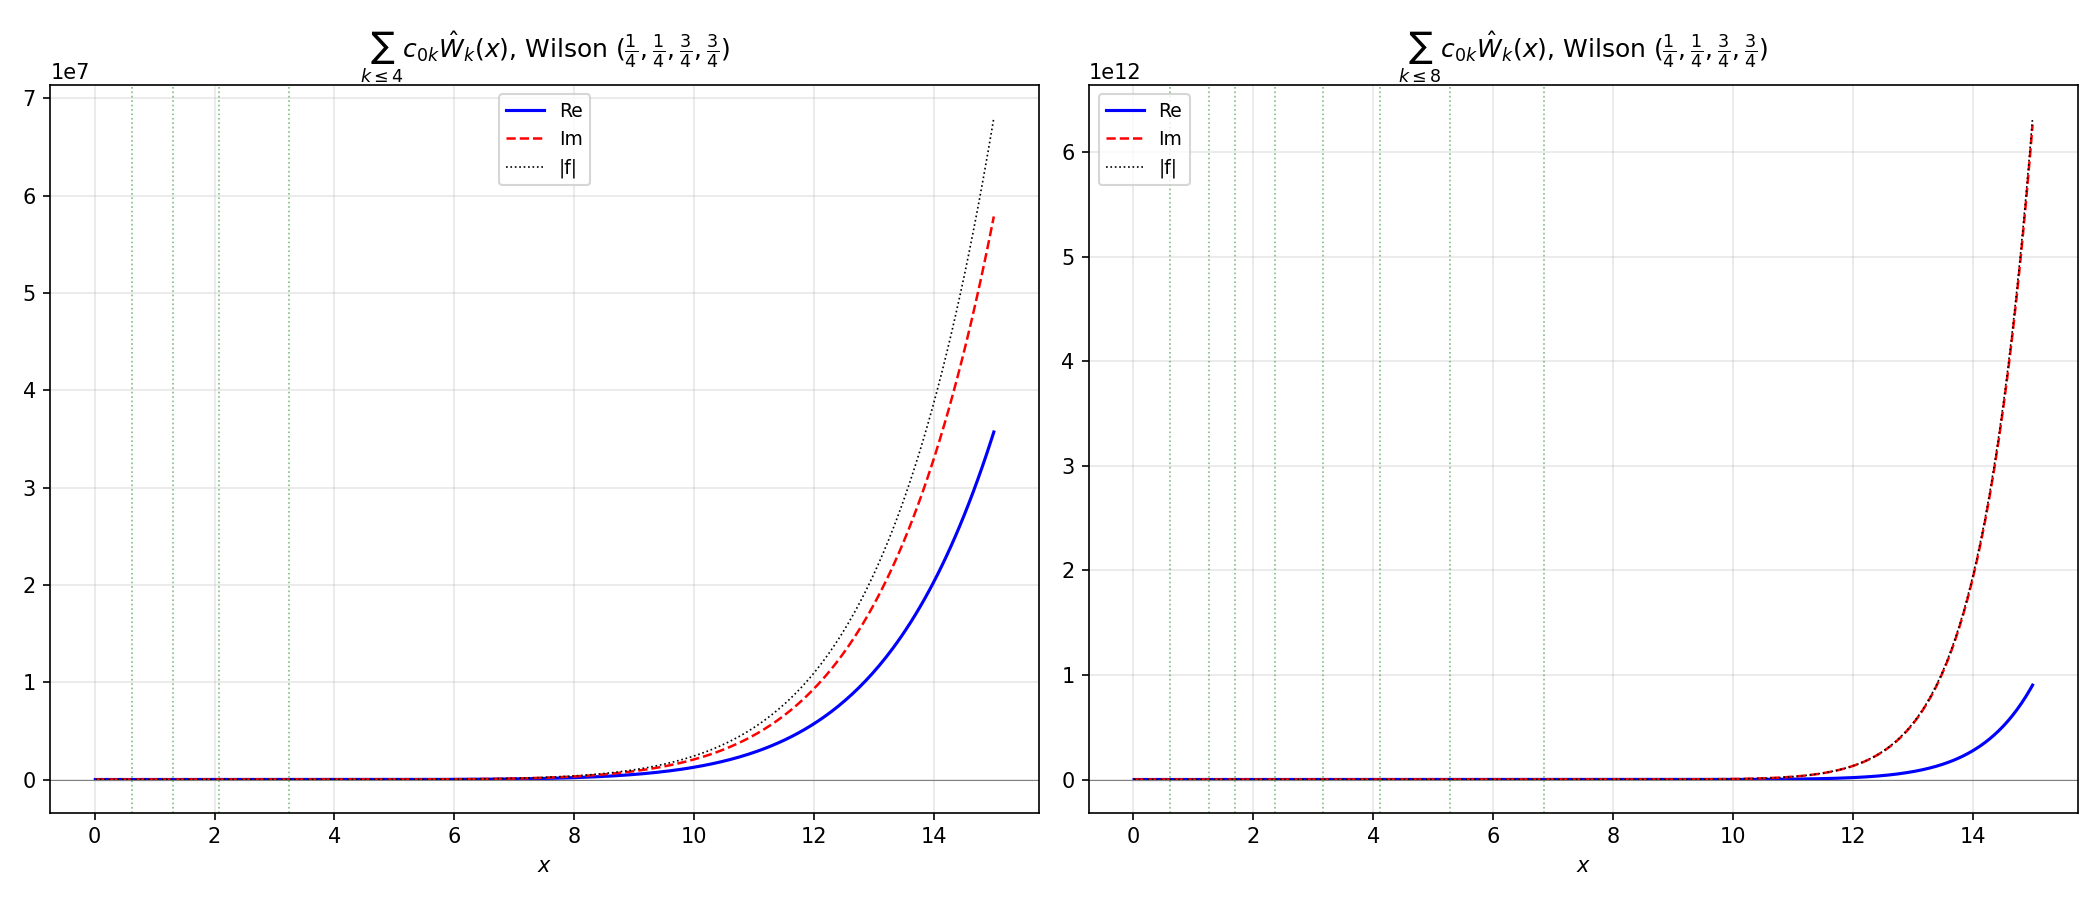
\includegraphics[width=0.95\textwidth]{wilson_zeros.png}
\caption{Truncated Wilson matching expansions $N = 4$ (left) and
$N = 8$ (right).  Green verticals mark real zeros of $\operatorname{Re} f$.}
\label{fig:zeros}
\end{figure}

The real zeros of $\operatorname{Re} f$ for $N = 8$ are
$x \approx 0.60, 1.26, 1.69, 2.37, 3.16, 4.11, 5.28, 6.85$.
The spacing increases linearly, consistent with the linear onset
prediction $x^* \sim (2N/\pi)\log(1/\rho)$ from the MP analysis
adapted to Wilson's $e^{-2\pi x}$ weight decay.

%% ===================================================================
\section{Summary}
%% ===================================================================

\begin{enumerate}
\item At $(\tfrac14,\tfrac14,\tfrac34,\tfrac34)$, the Pochhammer-free
Wilson polynomials have \emph{constant} norm $h_n = \pi^2$ for all~$n$
--- a Wilson-level identity.

\item The matching integral $c_{00}$ has net $9$ Gamma factors, exceeding
all known Barnes-type evaluations.  The $\Gamma(2ix)$ denominator
(coefficient~$2$) is the precise structural obstruction.

\item PSLQ (coefficients up to $10^4$, two-constant search over $11$
candidates) finds no algebraic relations: the Wilson matching
coefficients are \emph{new transcendentals}, not reducible to the
$\Q A \oplus \Q B$ ring of the MP case.

\item Both $b_{0k}$ and $c_{0k}$ decay as \textbf{power laws}
($\alpha \approx 1.4$ and $0.6$ respectively), consistent with
finite-distance poles of the weight.

\item The degeneration Wilson $\to$ MP is confirmed structurally
(the $\Gamma(2ix)$ obstruction cancels), though numerical verification
of the rescaled limit requires the intermediate continuous Hahn case.

\item Zeros of the truncated expansion show linearly increasing spacing,
paralleling the MP prediction.
\end{enumerate}

\end{document}
